% ----------------------------------------------------------
\chapter{Fundamentação teórica}\label{cap:fundteo}
% ----------------------------------------------------------
    Neste capítulo serão abordados os principais aspectos teóricos utilizados neste trabalho.

    \section{Diferença entre \ia, \am e \ap}
    
        Os temas \ia, \gls{ML}\footnote{Acrônimo do inglês para \ml.} e \gls{DL}\footnote{Acrônimo do inglês para \dl.} são discutidos assiduamente em estudos e vendidos como diferencial de produtos. Portanto nesta seção será definida cada uma dessas áreas e subáreas, apresentando suas diferenças. %nos meios de comunicação,
    
        A \ia, se propõe elaborar dispositivos que simulem a capacidade humana de raciocinar, perceber, tomar decisões e resolver problemas. Logo, qualquer técnica que permita computadores simular o comportamento humano pode ser definida com uma AI \cite{DeepLearningArtigo}. 
    
        \am é um subárea de AI. Seu intuito é fazer que as máquinas aprendam sozinhas usando dados fornecidos e assim, consigam realizar previsões com uma dada incerteza. Dentre os algorítimos de ML existe um outro subconjunto conhecido como \ap\textit{ }focado em \gls{NN}\footnote{Acrônimo do inglês para \nn.} \cite{kim2017matlab} .  
        
        As \rns\textit{ }são uma forma de modelar matematicamente sistemas de neurônios biológicos, e utiliza-los para resolver tarefas que outros tipos de algoritmos não conseguem realizar, por exemplo, classificação de imagens. Os subconjuntos de que compõem a AI podem ser visualizados na Figura~\ref{fig:AI_Ml_DL}.
            
        \begin{figure}[H]
            \centering
            \caption{Esquemático dos subconjuntos da AI.}
            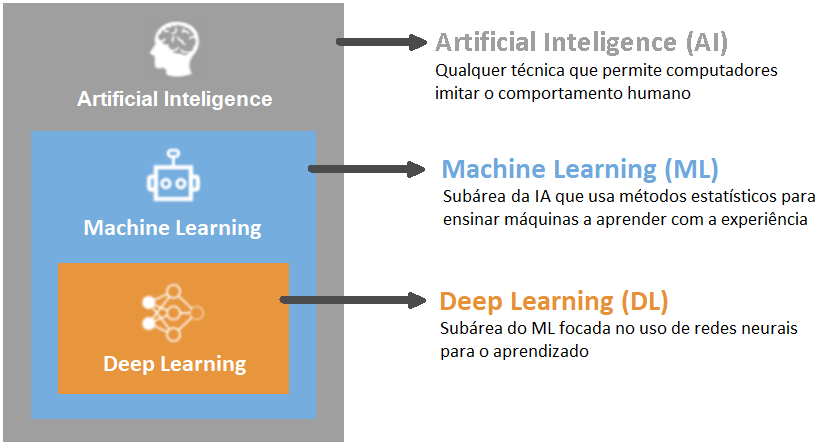
\includegraphics[width=0.7\textwidth]{fig/2-fundamentacao/diferenca_AI_ML_DL/Areas.png}
            \fonte{adaptado de \cite{site:RevolucaoIA}.}
            \label{fig:AI_Ml_DL}
        \end{figure}
        
        A ideia de \ap\textit{ }ser um "tipo"\textit{ }de \am\textit{ }é muito importante, e este é o motivo de realizar uma revisão sobre como AI, ML e DL estão relacionados. O \ap, por ter resolvido com proficiência alguns problemas que desafiaram a \ia\textit{ }esta em destaque recentemente. Seu desempenho, a pesar de ser excepcional em muitos campos, também enfrenta limitações que derivam de seus conceitos fundamentais os quais foram herdados de seu antecessor o ML. Como uma subárea do aprendizado de máquina, o aprendizado profundo não pode evitar os problemas base que o ML enfrenta. Por isso que é necessário apresentar o \am\textit{ }antes de discutir o conceito de \ap, o que será feito na seção~\ref{cap:ML}, porque o ML é alicerce do DL. 
        
    \section{Aprendizado de Máquinas}\label{cap:ML}
        
        Uma outra forma de compreender as técnicas de \am, é entendê-lo como método de análise de dados que visa automatizar a construção de modelos analíticos. Seus algoritmos são capazes de aprender iterativamente com os dados, possibilitando que computadores encontrem \textit{insights} sem serem explicitamente programados sobre onde e o que procurar nas informações \cite{CollegeL30:online}.
        
        Posto isso, nesta seção serão apresentadas as terminologias básicas necessárias em \am, como se dá o aprendizado e de que forma seus erros são reduzidos. Também será discutida a diferença entre tarefas supervisionadas e não supervisionadas, assim como a distinção entre classificação e regressão. No final, serão descritas as métricas de avaliação de performance de modelos de classificação.
        
        \subsection{Terminologias Fundamentais de ML e Introdução a Conceitos Básicos}
        
            Nesta subseção serão definidas terminologias fundamentais de \am e \ap obtidas em \cite{MachineL6:online}. A partir disso, é possível determinar conceitos como: tipos de tarefas, diferenças entre treinamento e inferência e assim por diante.
    
            Há dois tipos de tarefas em \am, as supervisionadas e as não supervisionadas. As tarefas supervisionadas aprendem como a combinar inputs para produzir previsões úteis sobre dados nunca antes vistos, ou seja, se tem conhecimento sobre qual é a saída para uma dada entrada \cite{singh2016review}. Já no caso de não ter noção prévia do que espera-se como inferência das redes, utiliza-se modelos não supervisionados.
        
            Duas terminologias muito importantes em \am\textit{ }supervisionada são os rótulos\footnote{Em inglês \textit{labels}.} e os atributos\footnote{Em inglês \textit{features}.} ). Os rótulos, são as classes e também o que se espera como predição do modelo, representado pela variável $y$. As atributos, são as variáveis de entrada (valores que caracterizam as amostras), representado por $x$. 
            
            Uma das formas de indicar o quão sofisticado é um projeto de aprendizado de máquinas é através da quantidade de atributos. Ou seja, redes que recebem como entradas poucos recursos são mais simples que as com múltiplas entradas. 
            
            Do conjunto de amostras, um exemplos é uma instância particular de dados do vetor de atributos $\mathbf{\overline{x}}$ e são classificados em duas categorias: exemplo rotulado\footnote{Em inglês \textit{labeled examples}.} e exemplo não rotulado\footnote{Em inglês \textit{unlabeled examples}.}. 
            
            Um exemplos rotulados incluí tanto atributo(s) como o rótulo(s). Ou seja:
            \begin{center}
                exemplos rotulados: \{atributo, rótulo\}: (x, y)
            \end{center}
    
            Já um exemplos não rotulados contem apenas as atributo(s) sem o rótulo(s). Como representado a seguir:
            \begin{center}
                exemplos não rotulados: \{atributo, ?\}: (x, ?)
            \end{center}
    
            Os problemas mais comuns resolvidos com este tipo de ML são os de regressão e classificação. Uma diferença entre eles, é que a regressão prediz valores contínuos, enquanto a classificação prediz valores discretos. Outra característica importante ocorre na forma de avaliar performance, com métricas específicas para cada um. Elas serão descritas na seção~\ref{cap:metrica}. 
            
            De tudo o que foi exposto até agora, é possível concluir que modelos de classificação e regressão necessitam de um banco de dados prévio, visto que utilizam exemplos com e sem rótulos, ou seja, são tarefas supervisionadas. Já no caso de aprendizado não supervisionado, que não se sabe a saída, exemplos comuns de aplicação são: problemas como detecção de anomalias (não se tem conhecimento do problema); agrupamentos individuais \footnote{Em inglês \textit{cluster}.}; e redução de dimensionalidade \cite{gentleman2008unsupervised}. Como este trabalho será sobre classificação de padrões sonoros, as técnicas de aprendizado supervisionado não serão abordadas.
            
            Para finalizar as definições básicas, necessita-se determinar o que é modelo, isso do ponto de vista de tarefas supervisionadas. Ele tem duas fases, que são:
    
            \begin{itemize}
                \item Treinamento: fase na qual o modelo aprende, ou seja, ele receberá exemplos rotulados e será permitido que ele gradualmente encontre a relação entre $x$ e $y$;
                \item Inferência: momento que será aplicado o modelo treinado em exemplos não rotulados, isto é, ele faz predições uteis ($y'$).
            \end{itemize}
    
    
        \subsection{Treinando modelo simples para compreender \am}\label{cap:ML_modelo_qualquer}
            
            A Figura~\ref{fig:dados_quaisquer} apresenta uma pequena amostra de dados observados, e a partir delas deseja-se encontrar uma relação entre $y$, variável de interesse dependente que se quer predizer, e $x$ a variável independente.
            
            \begin{figure}[H]
                \centering
                \caption{Pequena amostra de dados quaisquer.}
                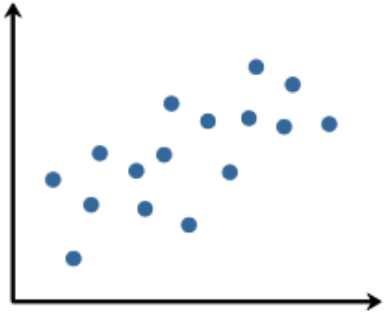
\includegraphics[width=0.3\textwidth]{fig/2-fundamentacao/treinar_modelo_simples/dados_quaisquer.png}
                \fonte{\cite{MachineL6:online}}
                \label{fig:dados_quaisquer}
            \end{figure}
            
            Pela análise da Figura~\ref{fig:dados_quaisquer} é possível dizer que, uma reta consegue inferir o comportamento entre $x$ e $y$, mesmo que não passe exatamente por todos os pontos, como a Figura~\ref{fig:dados_quaisquer_regressao} demonstra. Matematicamente é descrita pela equação~\ref{eq:reta} na convenção estabelecida em ML e adicionando o subíndice que indica a possibilidade de ter mais de uma dimensão. Para inferir $y$, basta substituir os valores de $x$ neste modelo (reta) \cite{CollegeL30:online}.
            
            \begin{equation}\label{eq:reta}
                \centering
                y' = b + w_{1}x_{1};
            \end{equation}
        
            em que:
            \begin{itemize}
                \item $y'$ é o rótulo predito \footnote{Em inglês \textit{predicted label}.} (saída desejado);
                \item $b$ é o bias (intercepção no eixo $y$);
                \item $w_{1}$ é o peso da atributo 1. Peso tem o mesmo conceito que a inclinação ($m$) tem na equação tradicional da reta;
                \item $x$ é o atributo (entrada).
            \end{itemize}
    
            \begin{figure}[H]
                \centering
                \caption{Regressão linear que prever o comportamento da pequena amostra de dados quaisquer.}
                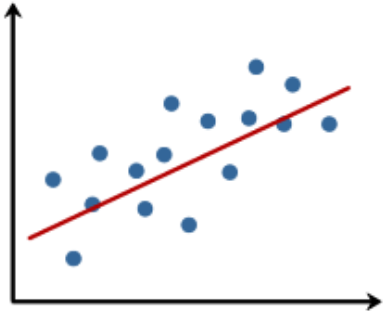
\includegraphics[width=0.3\textwidth]{fig/2-fundamentacao/treinar_modelo_simples/dados_quaisquer_regrassao.png}
                \fonte{\cite{MachineL6:online}}
                \label{fig:dados_quaisquer_regressao}
            \end{figure}
            
            O exemplo proposto considerar somente uma dimensão de atributos como entrada, ao contrário de modelo mais sofisticado que utilizam muito mais, e com isso, possuem mais pesos ($w$). Logo, há um peso para cada atributo em separado, como descreve a equação~\ref{eq:reta_varias_features}. 
            
            \begin{equation}
                \centering
                y' =  b + w_{1}x_{1} + w_{2}x_{2} + ... + w_{n}x_{n}.
                \label{eq:reta_varias_features}
            \end{equation}
            
            Para sintetizar, os dados foram aplicados em um algoritmo de \am e como resultado obteve-se um modelo, que neste caso é uma reta. Mas é gerada uma a pergunta: como o treinamento realmente acontece? Ele ocorre ao determinar bons valores para o bias e todos os pesos utilizando exemplos rotulados. Para isso, o algoritmo examina varias amostras, e compara a predição feita pela equação criada, com o valor real, buscando encontrar um modelo que minimize a perda entre $y$ e $y'$.
            
            A perda é também conhecida como erro, que é dado por um número que indica o quão boa foi a inferência de um exemplo único. Ele pode ser visto como uma penalidade dada ao modelo por fazer uma predição ruim. Se $y'$ for igual a $y$, a perda será zero, caso contrário, será um valor maior que zero e grande. 
            
            A Figura~\ref{fig:loss_learning} apresenta dois modelos, sendo que o da esquerda possui um erro alto. Uma forma de concluir isso, é através da distância muito maior entre a linha azul (equação) e o ponto (valor verdadeiro). No gráfico da direta esse espaço é pequeno, mostrando que a perda é menor.
    
            \begin{figure}[H]
                \centering
                \caption{O gráfico da esquerda ilustrar um modelo com alta perda e o da direita com baixa perda.}
                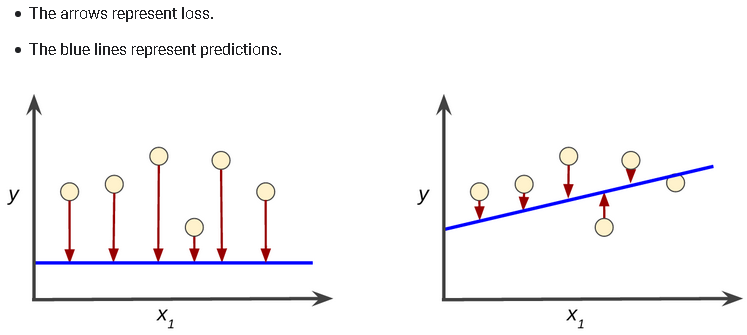
\includegraphics[width=0.7\textwidth]{fig/2-fundamentacao/aprendizado/loss_learning.png}
                \fonte{\cite{MachineL6:online}}
                \label{fig:loss_learning}
            \end{figure}
            
             Portanto o objetivo dos algoritmos de ML e DL é treinar o modelo para encontrar os valores de $w_i$ e $b$ que minimize essa diferença ao longo de todos os exemplos. A equação mais comum usada para esse cálculo é erro quadrático\footnote{Em inglês \textit{squared loss}.} , entretanto, ela é usada a partir do valor médio, denominado \gls{MSE}\footnote{Acrônimo do inglês para \textit{Mean square Error}.}, e descrito pela equação~\ref{eq:MSE}\cite{TotalTen29:online}.
            
            \begin{equation}
                \centering
                MSE =  \frac{1}{N} \sum_{(x,y)\in D}  (y - y')^2
                \label{eq:MSE}
            \end{equation}
        
            
            em que:
            \begin{itemize}
                \item $(x,y)$ é um exemplo no qual
                \begin{itemize}
                    \item $x$ é o conjunto de atributos que o modelo usa para realizar predições;
                    \item $y$ é o rótulo do exemplo.
                \end{itemize}
                \item $y'$ é a função de pesos e bias em combinação com o conjunto de atributos $x$;
                \item $D$ é um conjunto de dados contendo muitos exemplos rotulados, nos quais $(x,y)$ são pares;
                \item $N$ é o número de exemplos em $D$.
            \end{itemize}
            
       \subsection{Redução de Perda}     
    
            O diagrama apresentado na Figura~\ref{fig:abordagem_iterativa}, demonstra como o modelo de aprendizado de máquina reduz a perda iterativamente para aprender. Esse processo começa com o algoritmo gerando um "palpite", ou seja, um valor para $b$ e $w_1$. Então, o erro é calculado através da equação~\ref{eq:MSE}. 
            
            As entradas, na estimativa da perda, são o conjunto de rótulos, $y$, e a inferência, $y'$, realizada pelo primeiro modelo utilizando o conjunto de atributos. Após é repetido este processo, entretanto com um novo palpite e da comparação entre os resultado obtidos, o algoritmo escolhe qual das tentativa obteve o menor erro.
    
            \begin{figure}[H]
                \centering
                \caption{Abordagem iterativa para o treinamento do modelo através da redução do erro.}
                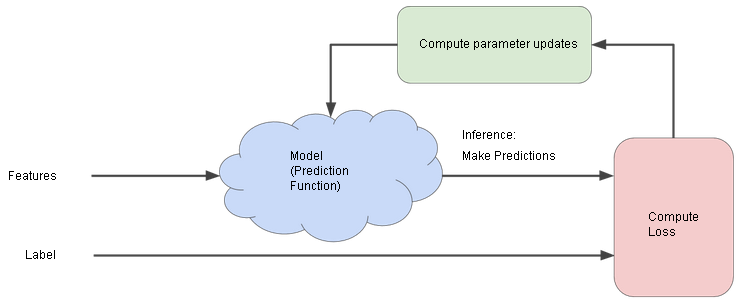
\includegraphics[width=0.8\textwidth]{fig/2-fundamentacao/aprendizado/abordagem_iterativa.png}
                \fonte{\cite{MachineL6:online}}
                \label{fig:abordagem_iterativa}
            \end{figure}
            
            O diagrama~\ref{fig:abordagem_iterativa} tem uma etapa chamada de \textit{Compute Loss}, que representa o momento no qual o algoritmo determina o erro. Na sequência, há o processo \textit{Compute Parameter Updates}, que caracteriza a rede e examina os valores calculados pela função de perda e escolhe como será a atualização deles. Esse procedimento de aprendizado continua a cada iteração até que o algoritmo descubra os parâmetros do modelo com a menor perda possível. 
            
            O ponto no qual o treinamento é interrompido é denominado ponto de corte, e é estabelecido a partir de um critério de parada. Normalmente determina-se esse momento na época na qual a perda geral para de mudar ou pelo menos mude de forma extremamente lenta, quando isso acontece, o modelo convergiu.
            
            Foi usado como exemplo um modelo de regressão linear, se para este caso forem calculados todos os valores possíveis de perda para $w_1$, o resultado seria sempre uma parábola com concavidade para cima. Ela é apresentada no gráfico convexo da Figura~\ref{fig:convexo}.
    
            \begin{figure}[H]
                \centering
                \caption{Problemas de regressão linear geram gráficos de perda vs $w_1$ (peso) convexo.}
                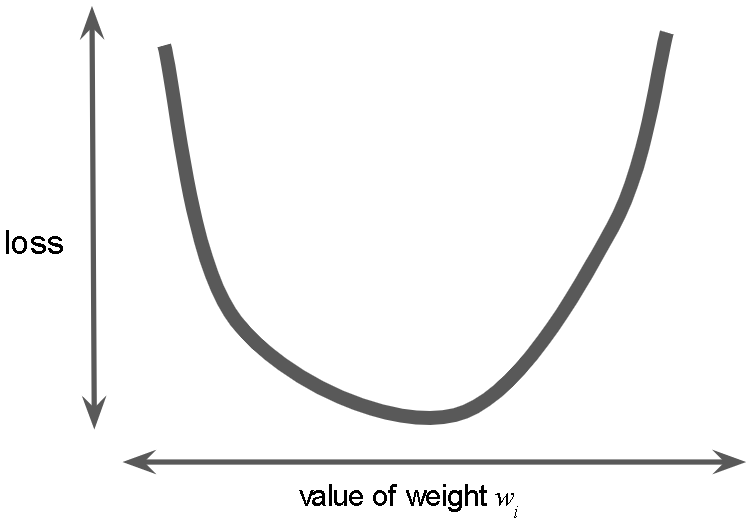
\includegraphics[width=0.435\textwidth]{fig/2-fundamentacao/aprendizado/convexo.png}
                \fonte{\cite{MachineL6:online}}
                \label{fig:convexo}
            \end{figure}
            
            Esse problema é muito simples, pois uma parábola possuí apenas um mínimo, ou seja, um ponto cuja inclinação é exatamente igual a 0. Entretanto, por mais fácil que seja visualizar o ponto onde a função perda converge em uma parábola, ainda é um processo inviável e ineficiente levantar todos os valores para posteriormente encontrar o mínimo.
            
            Um método melhor e mais popular, no aprendizado de máquinas, é o gradiente descendente. Essa técnica também começa com um palpite para $b$ e $w_1$. O ponto de partida não importa muito, assim, muitos algoritmos simplesmente configuram para iniciar em 0 ou em um valor aleatório, como exemplo, a Figura~\ref{fig:gradiente_descendente_ponto_inicial}. 
    
            \begin{figure}[H]
                \centering
                \caption{Ponto de partida aleatório utilizado pelo gradiente descente para minimizar a perda.}
                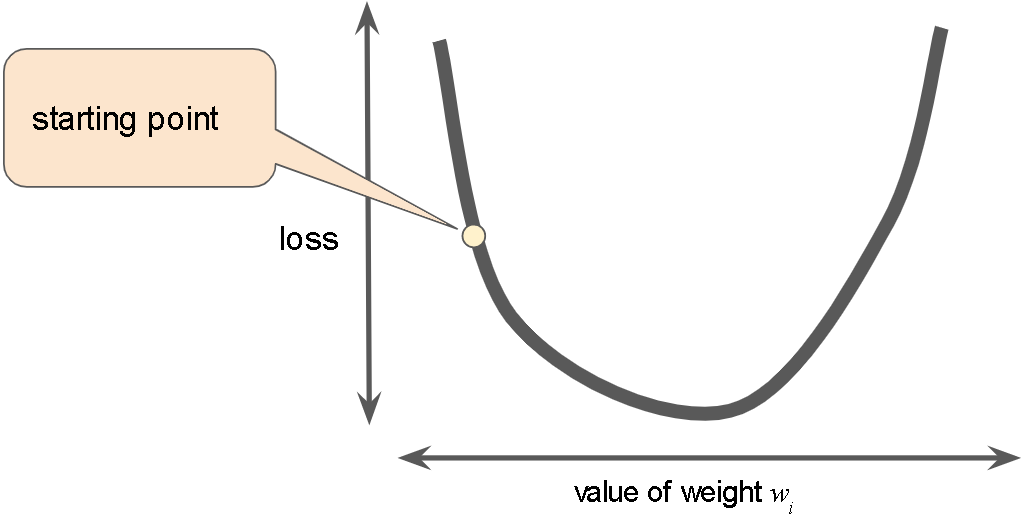
\includegraphics[width=0.6\textwidth]{fig/2-fundamentacao/aprendizado/gradiente_descendente_ponto_inicial.png}
                \fonte{\cite{MachineL6:online}}
                \label{fig:gradiente_descendente_ponto_inicial}
            \end{figure}
            
            O algoritmo calcula o erro no ponto inicial pela derivada parcial, que informa o quanto a função muda quando é feita uma pequena perturbação em uma variável com dado peso. Com base nesta variação, o gradiente consegue predizer se a inclinação da derivada é positiva ou negativa. Como o intuito é encontrar o mínimo, a rede seguirá o gradiente negativo, conhecido como gradiente descendente. Quando há vários pesos, o gradiente é um vetor de derivadas parciais em relação aos pesos. Como o gradiente é um vetor, ele tem uma direção e uma magnitude e seu resultado sempre aponta na direção do gradiente negativo para reduzir a perda o mais rápido possível, como mostra a Figura~\ref{fig:vetor_direcao_gradiente}. 
    
            \begin{figure}[H]
                \centering
                \caption{A descida do gradiente depende de gradientes negativos.}
                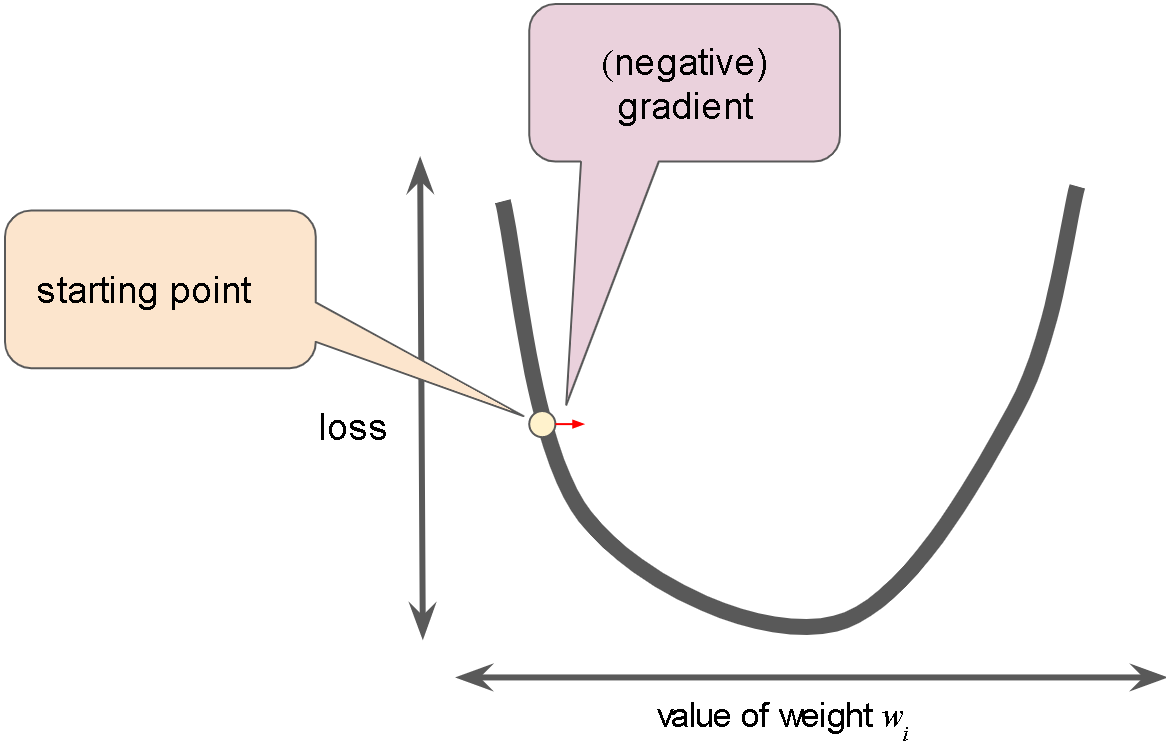
\includegraphics[width=0.6\textwidth]{fig/2-fundamentacao/aprendizado/vetor_direcao_gradiente.png}
                \fonte{\cite{MachineL6:online}}
                \label{fig:vetor_direcao_gradiente}
            \end{figure}
            
            Para determinar o próximo ponto ao longo da curva de perda, o algoritmo adiciona uma fração da magnitude do gradiente ao ponto inicial, conforme mostrado na Figura~\ref{fig:vetor_magnitude_gradiente}. Esse processo é repetido, chegando cada vez mais perto do mínimo. 
    
            \begin{figure}[H]
                \centering
                \caption{Acréscimo da magnitude do gradiente no valor do ponto inicial move para o próximo ponto da curva de perda.}
                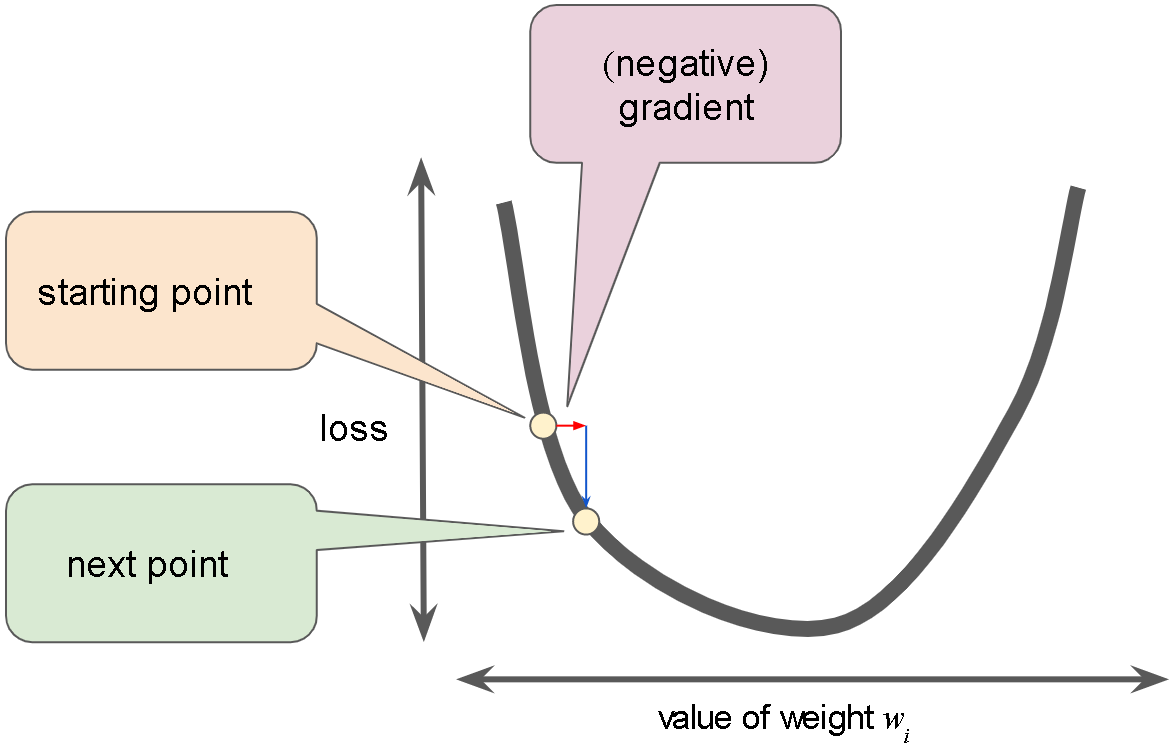
\includegraphics[width=0.6\textwidth]{fig/2-fundamentacao/aprendizado/vetor_magnitude_gradiente.png}
                \fonte{\cite{MachineL6:online}}
                \label{fig:vetor_magnitude_gradiente}
            \end{figure}
            
            Entretanto, não é somente somado ao ponto inicial o valor da magnitude. Antes disso, ela é multiplicada pala taxa de aprendizado, também chamado de tamanho do passo. A taxa de aprendizado é um hiper parâmetro, ou seja, uma das variáveis que controla o próprio processo de treinamento. Esse conjunto soma e multiplicação que realmente dita o próximo ponto de análise na função de perda. Para exemplificar, pode-se considerar uma magnitude de 2,5 e uma taxa de 0,01. O algoritmo escolherá o próximo ponto a uma distancia de 0,025 do valor anterior.
            
            A taxa de aprendizado trás algumas informações importantes: se ela for muito pequena, o treinamento demorará muito como mostra a Figura~\ref{fig:taxa_pequena}. Por outro lado, se ela for muito grande, o ponto irá saltar perpetuamente ao acaso perto do vale sem convergir, demonstrado pela Figura~\ref{fig:taxa_grande}. 
    
            \begin{figure}[H]
                \centering
                \caption{Se a taxa de aprendizagem for muito pequena a proximidade entre os passos é maior.}
                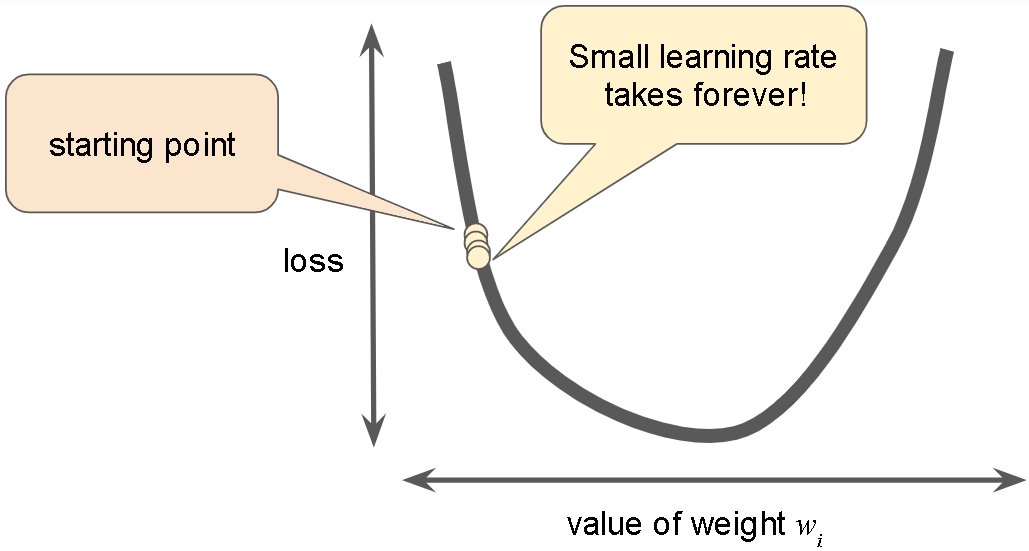
\includegraphics[width=0.6\textwidth]{fig/2-fundamentacao/aprendizado/taxa_pequena.png}
                \fonte{\cite{MachineL6:online}}
                \label{fig:taxa_pequena}
            \end{figure}
            
            \begin{figure}[H]
                \centering
                \caption{A taxa de aprendizagem é muito grande.}
                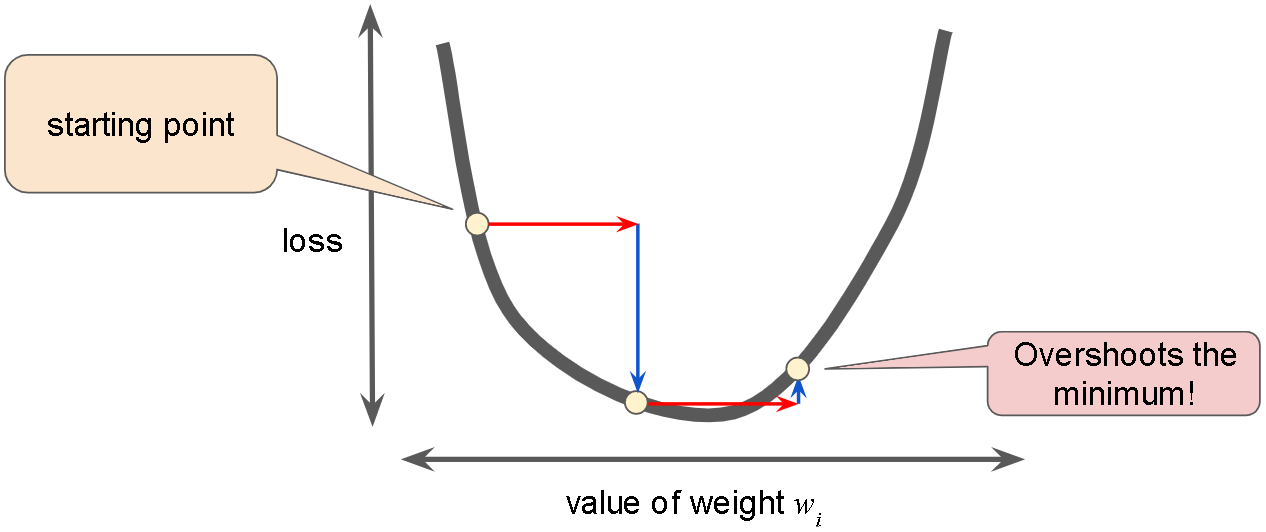
\includegraphics[width=0.6\textwidth]{fig/2-fundamentacao/aprendizado/taxa_grande.png}
                \fonte{\cite{MachineL6:online}}
                \label{fig:taxa_grande}
            \end{figure}
            
            Existe uma taxa de aprendizagem \textit{Goldilocks}\footnote{Em \rns\textit{ }é a taxa de aprendizado ideal.} para cada problema de regressão, que descreve o quão plana é a função de perda. Essa informação permite aumentar com segurança a taxa de aprendizado, se for de conhecimento prévio que o gradiente é pequeno. Com essa compreensão que o valor da magnitude do gradiente é pequeno, é possível configurar um tamanho de passo maior, e dessa forma, que a perda encontre o mínimo no menor número de etapas. Já a taxa de aprendizagem ideal em uma dimensão é o inverso da segunda derivada de $f(x)$ em $x$ e para 2 ou mais dimensões é o inverso da matriz das derivadas parciais secundárias. 
            
            Uma terminologia importante, no gradiente descendente, é lote\footnote{Em inglês \textit{batch}.} definido como o número total de exemplos usados para calcular o gradiente em uma única iteração. Quando é dado como entrada para o cálculo da inclinação o conjunto inteiro de dados, considera-se que foi utilizado um lote. Entretanto, eles geralmente contêm um grande número de atributos, ou seja, um lote pode ser enorme, fazendo com que até mesmo uma única iteração demore muito para ser computada.     
            
        \subsection{Generalização em modelos}
        
            Para descrever o que significa um modelo sobre-ajustado\footnote{Em inglês \textit{overfitting}}, um modelo sub-ajustado\footnote{Em inglês \textit{underfitting}} e o porquê de separar os dados em subconjuntos, serão usadas outras amostras com somente um atributo, apresentadas na Figura~\ref{fig:dados_simples}. Assim como no exemplo da seção anterior~\ref{cap:ML_modelo_qualquer}, o objetivo é desenvolver um modelo para prever os rótulos e a partir dele discutir esses processos \cite{kim2017matlab}.
    
            \begin{figure}[H]
                \centering
                \caption{Pequena amostra de dados com somente uma dimensão atributos.}
                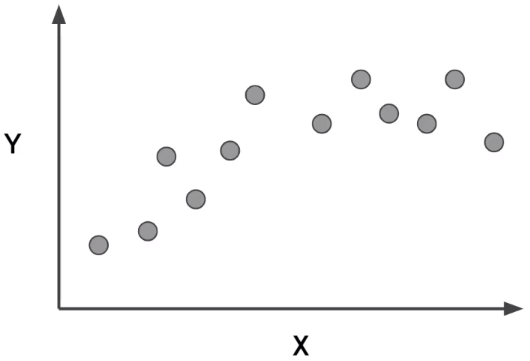
\includegraphics[width=0.5\textwidth]{fig/2-fundamentacao/overfitting/dados_simples.png}
                \fonte{\cite{Complete79:online}}
                \label{fig:dados_simples}
            \end{figure}
    
            É considerado como um bom modelo aquele que tenta se ajustar à tendência geral do conjunto de dados real, e não se encaixar perfeitamente neles. A Figura~\ref{fig:modelo_bom} exibe esse comportamento de generalizar seus resultados.
    
            \begin{figure}[H]
                \centering
                \caption{Comportamento esperado para um bom modelo.}
                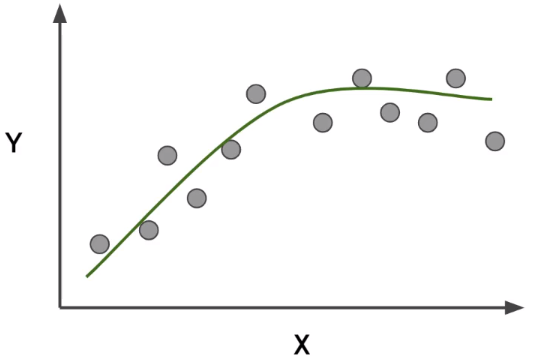
\includegraphics[width=0.5\textwidth]{fig/2-fundamentacao/overfitting/modelo_bom.png}
                \fonte{\cite{Complete79:online}}
                \label{fig:modelo_bom}
            \end{figure}
            
            A Figura~\ref{fig:overfitting} apresenta o comportamento de um  modelo com sobre-ajuste utilizando as amostras da Figura~\ref{fig:dados_simples}. Nela é possível ver que a curva passa exatamente em todos os pontos do gráfico. Quando isso acontece, ele se torna mais complexo do que necessário, seu erro de treinamento é extremamente baixo ou, como neste caso específico, igual à zero.
            
            \begin{figure}[H]
                \centering
                \caption{Modelo considerado ruim com a presença de sobre-ajuste.}
                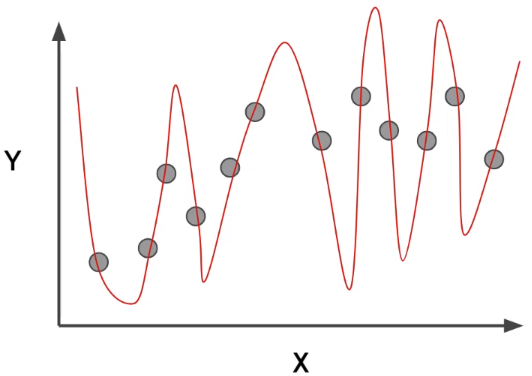
\includegraphics[width=0.5\textwidth]{fig/2-fundamentacao/overfitting/overfitting.png}
                \fonte{\cite{Complete79:online}}
                \label{fig:overfitting}
            \end{figure}
            
            O oposto do sobre-ajuste é o sub-ajuste, que ocorre em modelos excessivamente simples os quais não conseguem capturar a tendência dos dados para prever seu comportamento. Como resultado, frequentemente, apresentam baixa variança e alto bias. Um exemplo é apresentado na Figura~\ref{fig:underfitting}, ele também foi baseados nas amostras da Figura~\ref{fig:dados_simples}.
            
            \begin{figure}[H]
                \centering
                \caption{Exemplo de um modelo considerado ruim por apresentar sub-ajuste.}
                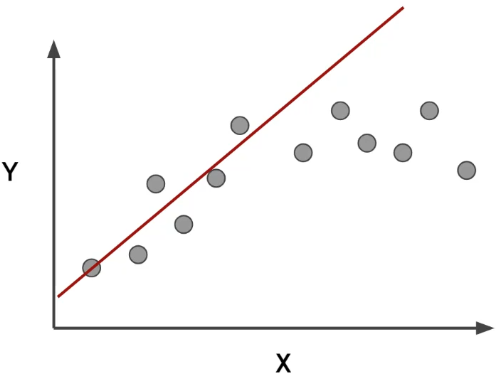
\includegraphics[width=0.5\textwidth]{fig/2-fundamentacao/overfitting/unterfitting.png}
                \fonte{\cite{Complete79:online}}
                \label{fig:underfitting}
            \end{figure}
            
            Infelizmente, o modelo não consegue considerar todas as informações possíveis, uma vez que ele só recebe uma amostra de dados, denominado conjunto de treinamento. Isso acarreta em um problema, se ocorrer sobre-ajuste ou sub-ajuste nos exemplos atuais, como confiar que o modelo também fará boas previsões sobre exemplos nunca antes vistos? Esse é o motivo de separar os conjuntos de dados em mais de um subconjunto. As separações mais utilizadas em ML são:
            
            \begin{itemize}
                \item Em duas divisões denominadas: treino e teste;
                \item Em três divisões denominadas: treino, teste e validação.
                % \item Em quatro divisões denominadas: treino, teste, validação e \textit{deployment}.
            \end{itemize} 
            
            O conjunto de teste deve atender à duas condições: ser grande o suficiente para produzir resultados estatisticamente significativos e ser representativo para o conjunto de dados como um todo. Em outras palavras, não pode ser escolhido um conjunto de teste com características diferentes do conjunto de treinamento. 
            
            Supondo que o conjunto de teste atenda às duas condições anteriores, independente de qual divisão for escolhida, haverá um subconjunto para testar o modelo já treinado. Dessa forma, é possível avaliar se há sobre-ajuste ou sub-ajuste a partir dos resultados do cálculo de erro. Isso porque esse valor será pequeno para o conjunto de treinamento, mas para as novas amostras de teste será muito maior. A Figura~\ref{fig:teste_overfitting_novo_valor} apresenta a um ponto de teste.
    
            \begin{figure}[H]
                \centering
                \caption{Novo valor teste aplicado a um modelo com sobre-ajuste.}
                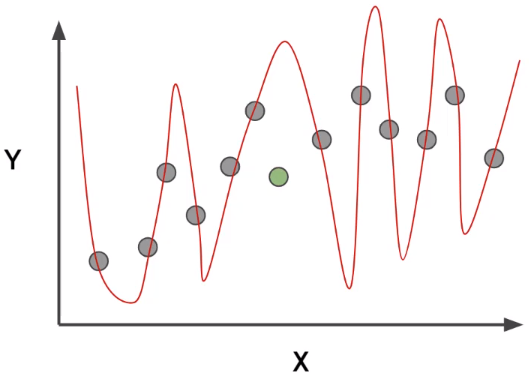
\includegraphics[width=0.5\textwidth]{fig/2-fundamentacao/overfitting/testando_overfitting.png}
                \fonte{\cite{Complete79:online}}
                \label{fig:teste_overfitting_novo_valor}
            \end{figure}
            
            A noção da grandeza do erro pode ser visualizada na distância entre o ponto, valor real, e a curva, equação de inferência, como mostras a Figura~\ref{fig:erro_novo_valor}. Lembrando que, os valores de teste não podem ser utilizados durante o treinamento, garantindo assim, que o modelo não tenha visto antes estes dados.
    
            \begin{figure}[H]
                \centering
                \caption{Apresenta distância entre o novo ponto e a predição do modelo, ou seja, uma visualização do erro.}
                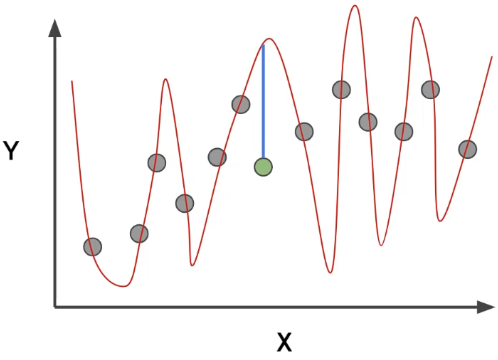
\includegraphics[width=0.5\textwidth]{fig/2-fundamentacao/overfitting/overfitting_erro_evaluate.png}
                \fonte{\cite{Complete79:online}}
                \label{fig:erro_novo_valor}
            \end{figure}
    
            Ao considerar a Figura~\ref{fig:teste_sem_overfitting}, nela esta representado o mesmo o modelo da Figura~\ref{fig:modelo_bom}, considerado bom, e o valor utilizado para teste na Figura~\ref{fig:teste_overfitting_novo_valor}. Por mais que o modelo seja muito simples e que não faça um trabalho perfeito (algumas previsões estão erradas), ele se sai tão bem nos dados de treinamento quanto no ponto de teste, ou seja, a equação não se ajusta demais nos dados de treinamento.
    
            \begin{figure}[H]
                \centering
                \caption{Mostra que a predição do modelo bom não seria perfeita, mas apresentaria um erro menor do que a com sobre-ajuste.}
                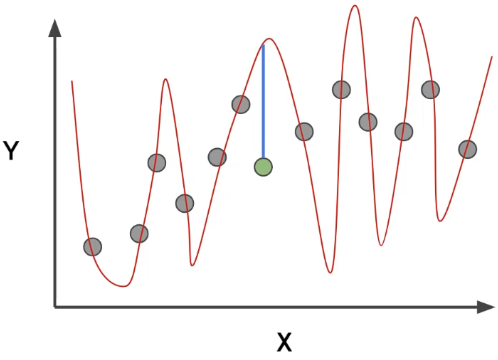
\includegraphics[width=0.5\textwidth]{fig/2-fundamentacao/overfitting/overfitting_erro_evaluate.png}
                \fonte{\cite{Complete79:online}}
                \label{fig:teste_sem_overfitting}
            \end{figure}
            
            Um bom desempenho no conjunto de teste, indica o quanto que se pode confiar nos resultados obtidos com novos dados. Entretanto, isso só é válido se o subconjunto de teste for grande o suficiente; e se não houver "trapaça", isto é, se o mesmo conjunto de teste não for usado repetidamente, ou no lugar do de treinamento. Esse último, pode-se ser concluído por métricas de avaliação com valores surpreendentemente bons, por exemplo, uma alta precisão pode indicar que os dados de teste vazaram para o conjunto de treinamento.
            
            Outra forma de garantir a qualidade dos resultados é eliminando exemplos que acarretam problemas de aprendizado para o algoritmo. Como no caso de um modelo treinado para classificar \textit{e-mails} como sendo spam ou não, o qual as amostras foram distribuídos em treino e teste. Indiferente do resultado, o esperado é obter valores para as métricas menores no conjunto de teste, isso porque o modelo não o usou como base de informações. 
            
            Na hipótese dele atingir a mesma acurácia nos dois conjuntos, treinamento e teste, gera-se um alerta. Logo, os dados devem ser verificados novamente, e se por acaso forem descobertos \textit{e-mail} duplicados entre os dois subconjuntos, a abordagem ideal é remover essas entradas e redividir as amostras. Do contrário, não será possível afirmar o quão bem o modelo consegue se generalizar realizando inferências  corretas sobre novos dados.     
            
            O fluxo de trabalho da divisão em dois conjunto, treino e teste, é ilustrado na Figura~\ref{fig:fluxo_treino_teste}. Nela, a etapa \textit{"Tweak model"} descreve o momento no qual pode-se ajustar a rede, e as possibilidades vão desde alterar a taxa de aprendizado, adicionar ou remover recursos, até projetar um modelo completamente novo do zero. No final deste fluxo de trabalho, escolhe-se o modelo que se sai melhor no conjunto de teste.
    
            \begin{figure}[H]
                \centering
                \caption{Fluxo de trabalho para separação do conjunto de dados em treino e teste.}
                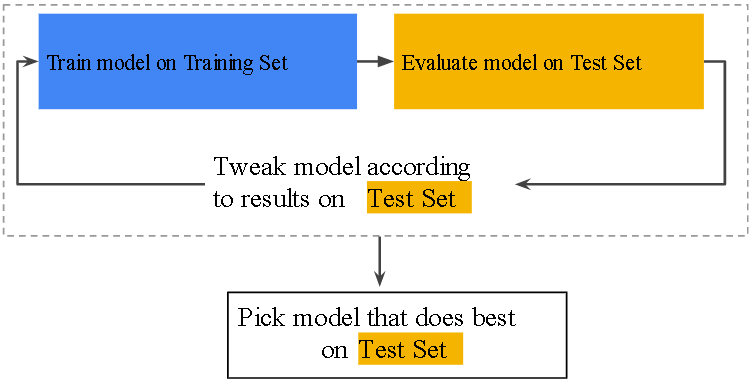
\includegraphics[width=0.7\textwidth]{fig/2-fundamentacao/overfitting/fluxo_treino_teste.png}
                \fonte{\cite{MachineL6:online}}
                \label{fig:fluxo_treino_teste}
            \end{figure}
            
            Entretanto, deve-se observar que esse procedimento é uma abordagem simplificada, pois a divisão é feita somente em dois blocos, o que não é adequado para obter o desempenho final do modelo. Isso porque é possível atualizar os parâmetros repetidas vezes após avaliar os resultados no conjunto de teste. Por causa disso, os dados costumam ser divididos em três conjuntos: treinamento, validação e teste.
            
            Essa abordagem reduz significativamente as chances de ocorrer sobre-ajuste, pois em resumo, as separações das amostra em 3 blocos são usadas da seguinte forma: com o conjunto para o treinamento o modelo consegue aprender as relações entre atributos e rótulos e assim ajustar-se aos dados. As amostras de validação são aplicadas à rede para verificar o desempenho e ele é a referência nos ajuste do modelo (adição de neurônios ou camadas, mudança na arquitetura real da rede etc.). Repete-se esse processo até ter resultados que satisfaçam condições específicas. Só então é possível avaliar a verdadeira performance do modelo com a ajuda da terceira divisão de dados, a de teste. Esse bloco é aplicado em métrica específicas para determinar o comportamento final, esperado em situações práticas. É importante observar que após executar o modelo com os dados de teste não será mais possível voltar e refinar os hiper-parâmetros da rede. O fluxo de trabalho da divisão em três conjunto é ilustrado na Figura~\ref{fig:fluxo_treino_teste_validação}.
    
            \begin{figure}[H]
                \centering
                \caption{Fluxo de trabalho para separação do conjunto de dados em treino, teste e validação.}
                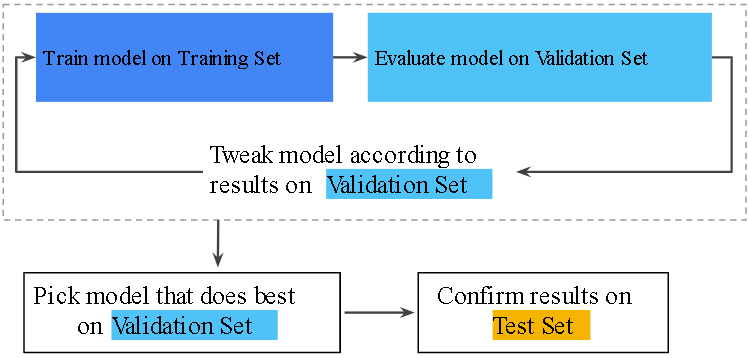
\includegraphics[width=0.7\textwidth]{fig/2-fundamentacao/overfitting/fluxo_treino_teste_validação.png}
                \fonte{\cite{MachineL6:online}}
                \label{fig:fluxo_treino_teste_validação}
            \end{figure}
            
            Até agora, as explicações foram realizadas com base em problemas de uma única atributos, pois são de fácil visualização. Entretanto, isso não ocorre frequentemente em situações práticas, em que a maior parte do tempo, trabalha-se com conjuntos de dados multidimensionais, o que exige uma abordagem diferente. Para discutir o melhor procedimento, pode-se considerar a Figura~\ref{fig:erro_tempo_treinamento} que apresenta a relação entre medição do erro e tempo de treinamento de um modelo considerado ideal.
            
            \begin{figure}[H]
                \centering
                \caption{Modelo ideal em relação ao erro versus tempo de treinamento.}
                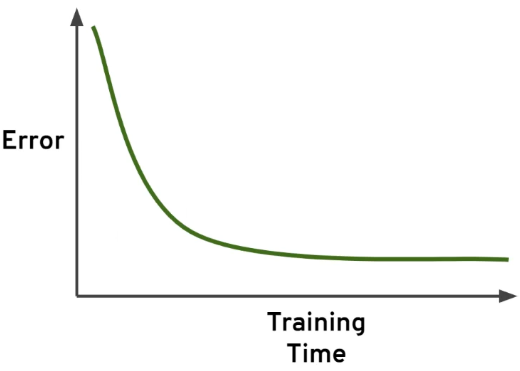
\includegraphics[width=0.5\textwidth]{fig/2-fundamentacao/overfitting/multidimencional_treinamento.png}
                \fonte{}
                \label{fig:erro_tempo_treinamento}
            \end{figure}
            
            Ao aplicar os dados de treinamento pela primeira vez no modelo, o valor de perda obtido será grande. Isso ocorre porque o algoritmo não teve acesso a essas informações antes e não ajustou quaisquer parâmetros internos como hipótese inicial. No entanto, conforme ocorre o aprendizado, ou seja, quanto mais tempo de treinamento, espera-se que o erro diminua até que se estabilize e convergindo para algum tipo de mínimo.
            
            No caso de redes neurais, este tempo de treinamento tem uma denominação específica, época\footnote{Em inglês epochs}. Essencialmente, uma época ocorre quando a totalidade dos dados de treinamento passa pelo modelo. Esse procedimento acontece várias vezes até que se obtém um bom modelo, como mostra a Figura~\ref{fig:epoch}. % erro convergirá para algum tipo de mínimo o
            
            \begin{figure}[H]
                \centering
                \caption{Modelo ideal em relação ao erro versus épocas.}
                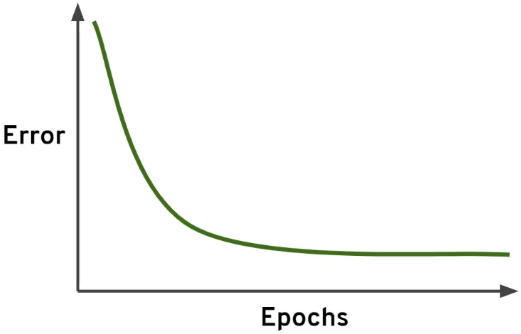
\includegraphics[width=0.5\textwidth]{fig/2-fundamentacao/overfitting/epoch.png}
                \fonte{\cite{Complete79:online}}
                \label{fig:epoch}
            \end{figure}
            
            Um modelo péssimo apresenta erros crescentes a medida que o tempo passa, ou seja, o modelo não aprende a cada época. Esse comportamento é demonstrado pela Figura~\ref{fig:modelo_ruim}.
            
            \begin{figure}[H]
                \centering
                \caption{Modelo ruim em relação ao erro versus épocas.}
                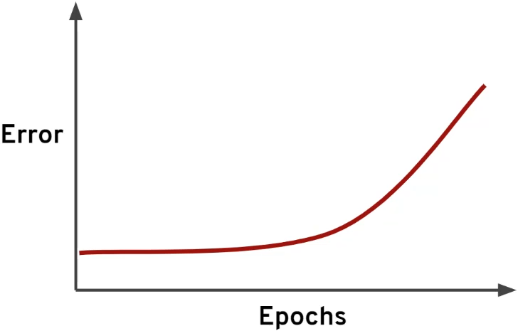
\includegraphics[width=0.5\textwidth]{fig/2-fundamentacao/overfitting/modelo_ruim.png}
                \fonte{\cite{Complete79:online}}
                \label{fig:modelo_ruim}
            \end{figure}
            
            Portanto, o estudo da simplicidade/complexidade dos modelos é importe para compreender a relação entre o desempenho deles nos conjuntos de treino e de teste/validação, sendo possível visualizar esse comportamento conforme as épocas passam. A Figura~\ref{fig:epocas_treino_teste} mostra os resultados ideais obtidos durante o treinamento, curva em vermelho, e de o teste, curva em azul.
            
            \begin{figure}[H]
                \centering
                \caption{Modelo ideal de erro de treino e de teste em relação ao as épocas.}
                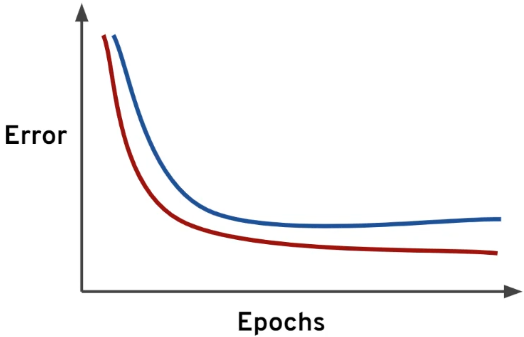
\includegraphics[width=0.5\textwidth]{fig/2-fundamentacao/overfitting/epocas_treino_teste.png}
                \fonte{\cite{Complete79:online}}
                \label{fig:epocas_treino_teste}
            \end{figure}
            
            No comportamento ideal, tanto o conjunto de treino como o de teste tem seu erro reduzido a medida em que as épocas passam. O resultado deles é similar, entretanto, no teste espera-se valores de perda maiores. Porém, se há sobre-ajuste, ao testa-los, tanto com os dados de teste como com os de validação, o resultado será ruim o que pode ser analisado na Figura~\ref{fig:Epoca_teste_ruim}.
            
            \begin{figure}[H]
                \centering
                \caption{Modelo ruim de erro de treino e de teste em relação ao as épocas.}
                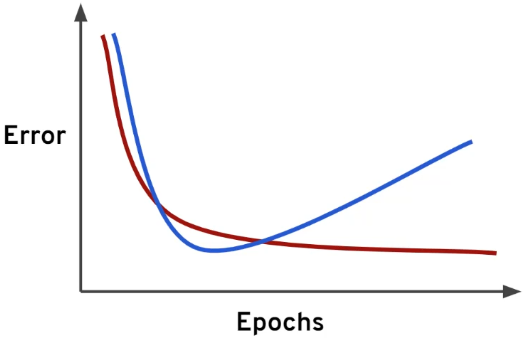
\includegraphics[width=0.5\textwidth]{fig/2-fundamentacao/overfitting/Epoca_teste_ruim.png}
                \fonte{\cite{Complete79:online}}
                \label{fig:Epoca_teste_ruim}
            \end{figure}
            
            O exemplo da Figura~\ref{fig:Epoca_teste_ruim} é uma boa indicação de complexidade excessiva nos dados de treino. Nela é possível visualizar o ponto no conjunto de teste, no qual o erro começa a aumentar ao invés de reduzir. Esse ponto define quando parar de treinar o modelo, pois, para as épocas a seguir começará o sobre-ajuste e os resultados para novos dados serão piores \cite{CollegeL30:online}. Esse ponto de corte é apresentado na Figura~\ref{fig:ponto_de_corte}.
            
            \begin{figure}[H]
                \centering
                \caption{Ponto de corte no tempo de treinamento para evitar sobre-ajuste.}
                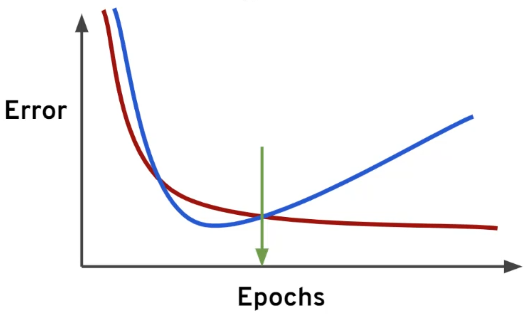
\includegraphics[width=0.5\textwidth]{fig/2-fundamentacao/overfitting/ponto_de_corte.png}
                \fonte{\cite{Complete79:online}}
                \label{fig:ponto_de_corte}
            \end{figure}
            
        \subsection{Avaliação de desempenho - Métricas de erro de classificação}\label{cap:metrica}
            
            Esta seção descreverá as métricas de avaliação de desempenho para problemas de classificação. Elas são utilizadas no final do processo de aprendizado, após o treinamento, com os dados do conjunto de teste e buscam avaliara eficiência do modelo. 
            
            As principais métricas de classificação estudadas por este trabalho são: acurácia, \textit{recall}, precisão e F1-Score. Antes de descrever-las, será explicado o raciocínio por trás delas e como realmente funcionam no mundo real. 
            
            Em uma típica tarefa de classificação, o modelo pode alcançar apenas dois resultados: ou ele realizou uma previsão correta; ou ele realizou uma previsão incorreta. Todas as métricas de classificação derivam dessa ideia, e felizmente, é possível expandi-la para situações em que há várias classes. Entretanto, para explicar o propósito delas será considerado uma classificação binária.
            
            A partir de um modelo que tem como objetivo classificar imagens como sendo de cachorro ou de gato, será descrito como determinar o desempenho real/final. O conjunto de teste possuí atributos, $x_{\text{test}}$, imagens de cachorro e gato, e seus respectivos rótulos, $y_{\text{test}}$, o nome cachorro e gato. 
            
            As imagens são dadas como entrada no modelo já treinado, que faz uma previsão. Esse resultado será uma predição correta, por exemplo, se a rede inferir cachorro para uma imagem de cachorro, como mostra a Figura~\ref{fig:cao_igual_cao}. 
            
            \begin{figure}[H]
                \centering
                \caption{Predição correta da rede neural.}
                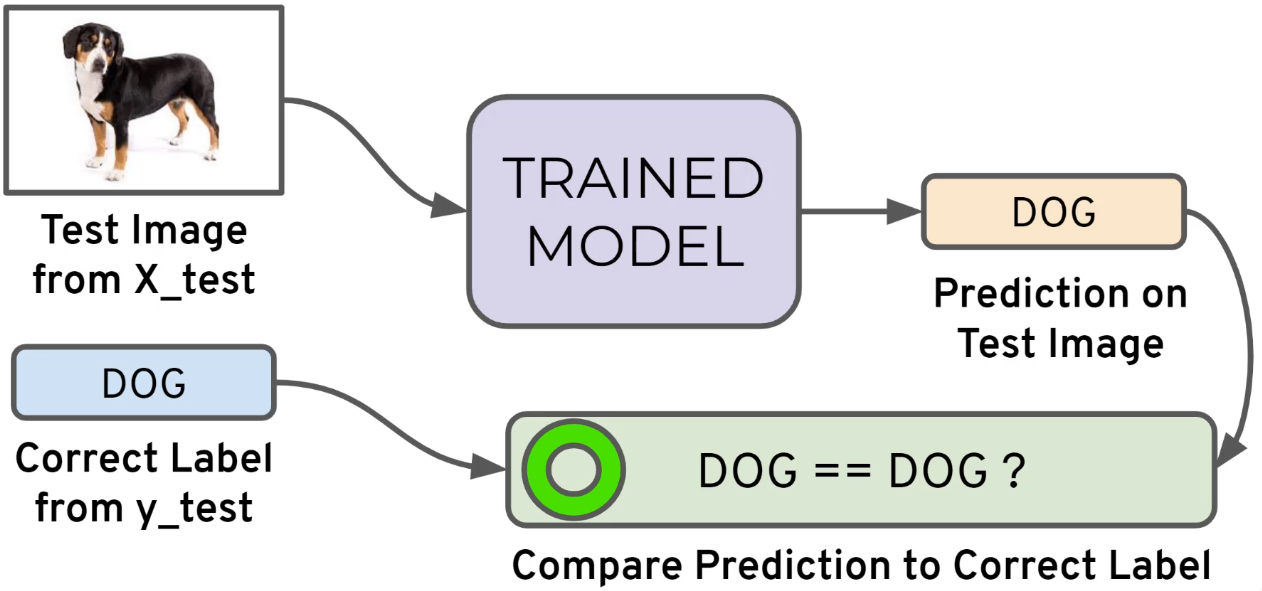
\includegraphics[width=0.5\textwidth]{fig/2-fundamentacao/metricas/cao_igual-cao.png}
                \fonte{\cite{Complete79:online}}
                \label{fig:cao_igual_cao}
            \end{figure}
            
            Porém, ela estará incorreta quando seu saída for gato e a imagem é de um cachorro, resultado apresentado pela Figura~\ref{fig:gato_nao_igual_cao}. 
        
            \begin{figure}[H]
                \centering
                \caption{Predição incorreta da rede neural.}
                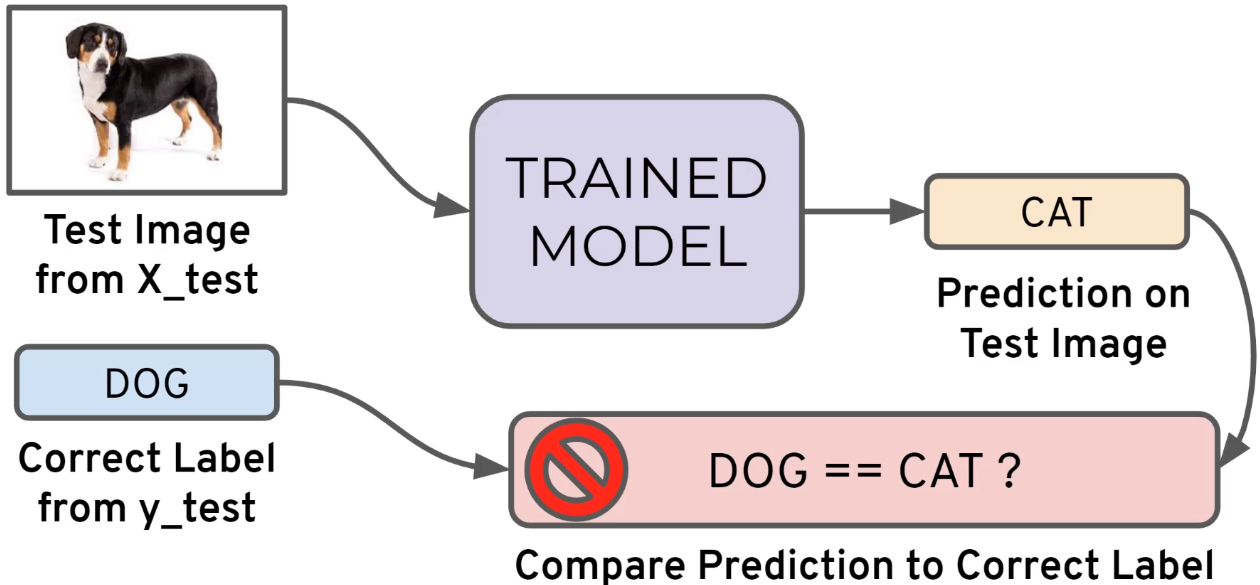
\includegraphics[width=0.5\textwidth]{fig/2-fundamentacao/metricas/gato_nao_igualcao.png}
                \fonte{\cite{Complete79:online}}
                \label{fig:gato_nao_igual_cao}
            \end{figure}
            
            Ao repetir esse processo para todas as imagens do banco de dados de teste, tem-se uma contagem das correspondências corretas e incorretas. É importante dizer que, no mundo real, nem todas as correspondências incorretas ou corretas têm o mesmo valor. Isso significa que uma única métrica não é o suficiente para caracterizar o desempenho do modelo. Portanto, são utilizados as quatro métricas e organiza-se os valores previstos em comparação com os reais no que é conhecido como matriz de confusão.
            
            A matriz de confusão apresenta os resultados de classificações corretas versus incorretas, como mostra a Figura~\ref{fig:matriz_confusão}. As condições verdadeiras (\textit{True Condition}) que indicam qual o rótulo correto/esperado para um dada inferência. Essas condições possuem duas subcategorias, positiva e negativa. Em outras palavras, é realmente cachorro versus não é, conforme Figura~\ref{fig:gato_nao_igual_cao}. As inferência realizadas pelo modelo são apontadas na condições de predição (\textit{Predicted Condition}), que também podem assumir duas categorias, positiva e negativa.
        
            \begin{figure}[H]
                \centering
                \caption{Matriz de confusão na qual computa predições em relação do que se esperava como \textit{output}.}
                \includegraphics[width=0.7\textwidth]{fig/2-fundamentacao/metricas/matriz_confusão.png}
                \fonte{\cite{Complete79:online}}
                \label{fig:matriz_confusão}
            \end{figure}
            
            Como é possível analisar, os elementos da diagonais da matriz apresentam as previsões corretas para diferentes classes, enquanto os dados fora da diagonal mostram as amostras que foram mal classificadas. Assim, as possibilidades de resultados de classificações são:
            \begin{itemize}
                \item Verdadeiro Positivo (\textit{True Positive} - TP): o modelo prediz corretamente a classe positiva;
                \item Verdadeiro Negativo (\textit{True Negative} - TN): o modelo prediz corretamente a classe negativa;
                \item Falso Positivo (\textit{False Positive} - FP): o modelo prediz incorretamente a classe positiva (erro tipo 1);
                \item Falso Negativo (\textit{False Negative} - FN): o modelo prediz incorretamente a classe negativa (erro tipo 2).
            \end{itemize}\\
            
            Considerando como classe positiva a imagem de cachorro e a negativa a de gato, tem-se os seguintes resultados:
            \begin{itemize}
                \item TP: é a imagem de um cachorro e o modelo predisse corretamente cachorro;
                \item TN: é a imagem de um gato e o modelo predisse corretamente gato;
                \item FP: é a imagem de um cachorro e o modelo predisse incorretamente gato;
                \item FN: é a imagem de um gato e o modelo predisse incorretamente cachorro;
            \end{itemize}
            
            A partir das informações discutidas até aqui, é possível compreender as métricas, começando pela acurácia, que pode ser calculada pela média dos valores situados na "diagonal principal". Neste caso, ela é escrita em termos de positivos e negativos como mostra a equação~\ref{eq:acuracia_positivo_negativo}.
            
            \begin{equation}
                \centering
                \text{Acurácia} = \frac{TP + TN}{TP + TN + FP + FN}
                \label{eq:acuracia_positivo_negativo}
            \end{equation}
            
            Frequentemente é definida como o número de previsões corretas feitas pelo modelo dividido pelo número total de predições, conforme a expressão~\ref{eq:acuracia}. Independente da forma escolhida para representa-la, a acurácia responde a pergunta, quantas predições corretas o modelo acertou em porcentagem. Por exemplo, um modelo terá uma acurácia de 80$\%$ se em um conjunto de testes com 100 imagens ele prever corretamente 80 delas. 
            
            \begin{equation}
                \label{eq:acuracia}
                \centering
                \text{Acurácia} = \frac{\text{Número de predições corretas}}{\text{Número total de predições}}
            \end{equation}
            
            O problema dessa métrica, é que ela é eficaz somente quando as classes alvo são bem balanceadas, isto é, sempre que há aproximadamente a mesma quantidade de imagens nas diferentes categorias. Mas em situações com desbalanceadas ela é péssima para determinar o desempenho. Para entender o significado disso, pode-se considerar um conjunto de teste com 99 imagens de cães e apenas uma de gato, e um modelo de uma linha que sempre irá prevê cachorro. A acurácia neste caso é de 99 $\%$, porque o único \textit{output} desta rede é cachorro, não importando a imagem dada a ela, e existem 99 imagens deles. Do contrário, se fosse uma reta constante na classe gato, o cálculo resultaria em 1 $\%$ de acurácia, pois existe somente uma imagem deste animal. O motivo de utilizar outras métricas é porque na maior parte das situações trabalha-se com desigualdade de rótulos.
            
            Entre as métricas utilizadas com classes desbalanceadas estão \textit{recall} e precisão. A primeira é definida como a capacidade de um modelo encontrar todos os casos relevantes dentro de um conjunto de dados, e sua definição precisa é dado pela equação~\ref{eq:recall}. Essa métrica tenta responder a pergunta: Qual proporção de positivos reais foi identificada corretamente? 
            
            \begin{equation}
                \centering
                Recall = \frac{TP}{TP + FN}
                \label{eq:recall}
            \end{equation}
            
            Já a precisão é a capacidade de um modelo de classificação identificar apenas os pontos de dados relevantes, sendo descrita matematicamente pela equação~\ref{eq:precisão}. O objetivo dela é responder a pergunta: Qual proporção de identificações positivas estava realmente correta?
            
            \begin{equation}
                \centering
                Recall = \frac{TP}{TP + FP}
                \label{eq:precisão}
            \end{equation}
            
            Constantemente, há a necessidade de encontrar o equilíbrio entre \textit{recall} e precisão. Para isso usa-se uma combinação delas que é conhecida como F1-Score. Ela é obtida através a média harmônica entre essas duas métricas, de acordo com a equação~\ref{eq:F1Score}. A F1-Score informa o quão preciso é o classificador, ou seja, quantas instâncias ele classifica corretamente, bem como, o quão robusto ele é, quer dizer, se ele não perde um número significativo de instâncias.
            
            \begin{equation}
                \centering
                F1-Score = 2\cdot\frac{\textit{precisão} \cdot recall}{\textit{precisão} + recall}
                \label{eq:F1Score}
            \end{equation}
            
            A razão para utilizar a média harmônica em vez da simples, é porque essa pune diferenças extremas. Por exemplo, se um classificador tem uma precisão igual à 1 (perfeita) e o \textit{recall} igual à zero (pior registro possível), com a média simples o resultado é igual a 0,5, já estimado com o F1-Score a solução é 0. Então, pode-se notar que F1-Score penaliza desproporções grandes de precisão e \textit{recall} e, portanto, é uma avaliação mais justa, principalmente para classes desbalanceadas. 
            
            A matriz de confusão e as várias métricas calculadas são maneiras de comparar o valor predito com o verdadeiro. Mas uma pergunta relevante é, qual dessas métricas é a "ideal"? A reposta depende da situação na qual o modelo está sendo executado, e do contexto do problema. Não existe um número único que possa afirmar o que é melhor. Por exemplo, não é possível declarar que $99\%$ de acurácia é bom o suficiente para todas as situações, já que para classes desbalanceadas isso não se aplica. A mesma observação vale para precisão e \textit{recall}, pois, ao ajustar o resultado para diminuir um, o outro será aumentado. Ou seja, é necessário decidir se o modelo deve se concentrar na correção de falsos positivos ou nos de falsos negativos. Essa constatação pode ser exemplificada ao substituir o exemplo da classificação de imagens por a de diagnóstico de doença. 
            
            No problema de predição de doenças, dificilmente haverá uma enfermidade que cerca de metade da população seja afetada e a outra não, logo, é um problema de classes desbalanceadas. Isso causa um "cobertor curto" entre precisão, que diminuindo melhora os FP, e \textit{recall}, que diminuindo melhora os FN. É importante ressaltar que, modelos de inteligência artificial, em situações de problemas de saúde são usados como diagnóstico rápido antes de realizar um exame mais invasivo, pois, na investigação de patologias mais severas, as "apostas" são altas. Neste caso, é melhor tentar minimizar o número de falsos negativos ao custo de aumentar o de falsos positivos. para se ter certeza de que foram classificados corretamente o maior quantidade possível de casos. 
            
            Portanto, o ideal nesta cenário é que todas as pessoas doentes passem para a próxima etapa, isso é muito importante, pois os modelos de inteligência artificial não são perfeitos. Dessa forma, é melhor diagnosticar uma pessoa como enfermar e garantir que ela siga sendo acompanhada para no futuro, com outros exames, possa ser dispensada como um diagnóstico errado, do que não tratar uma pessoa enferma. Isso considerando que haverão testes complementares, que por mais invasivos possam confirmaram ou não esse resultado prévio. O oposto é verificado na fabricação de equipamento, onde prefere-se que máquinas sem defeito sejam descartadas (FP) do que as com mau funcionamento sejam entregues ao consumidor final (FN).
            
            Existem outras métricas calculáveis que tentam prever o desempenho de modelos, entretanto, este trabalho irá abordar somente as descritas neste capítulo. Para mais informação sobre outras possibilidade de determinar a performance podem ser estudadas em\todo{citar bibliografia wikipédia}. 
        
            
        \subsection{Regressão logística para classificação binária}
        
            Muitos problemas requerem uma estimativa de probabilidade como saída. A regressão logística é um mecanismo extremamente eficiente para o cálculo de probabilidades. Em termos práticos, pode-se usar o resultado da probabilidade de uma das seguintes maneiras: como é; ou convertido em uma categoria binária.
            
            Usando sem alteração, "como está", é calculado pela probabilidade de $A$ ocorrer dado $B$, definido por~\ref{eq:probabilidade_A|B}.
            
            \begin{equation}
                \centering
                p(A|B)
                \label{eq:probabilidade_A|B} 
            \end{equation}
            
            É possível converter o resultado da probabilidade para um valor binário, ou seja, para uma classificação (tema deste trabalho). Isso é realizado a partir de um limiar, também conhecido por limite de decisão, que define quando um valor de probabilidade passa de uma categoria para outra.
            
            Para garantir que a saída do modelo de regressão logística fique entre 0 e 1, é usado uma função sigmoide, que produz o seguinte gráfico, apresentado na Figura~\ref{fig:sigmoide}. 
        
            \begin{figure}[H]
                \centering
                \caption{Função sigmoide.}
                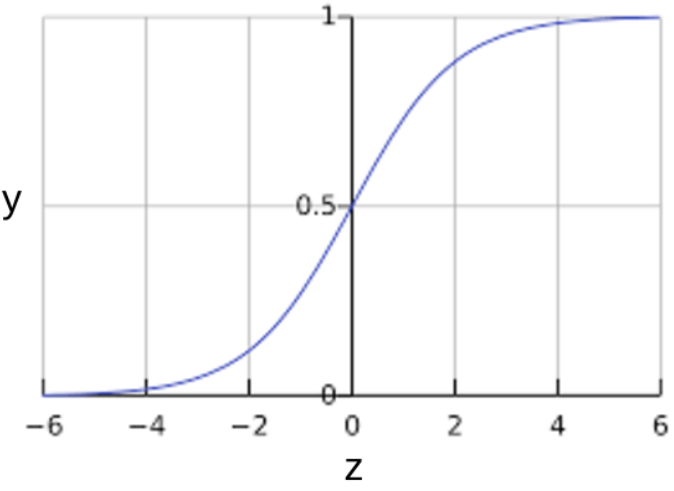
\includegraphics[width=0.5\textwidth]{fig/2-fundamentacao/aprendizado/sigmoide.png}
                \fonte{\cite{MachineL6:online}}
                \label{fig:sigmoide}
            \end{figure}
            
            Se $z$ representa a saída da camada linear de um modelo treinado com regressão logística, então sigmoide ($z$) produzirá um valor (uma probabilidade) entre 0 e 1, dado pela equação~\ref{eq:sigmoide}. 
            
            \begin{equation}
                \label{eq:sigmoide}
                \centering
                y = \frac{1}{1 + \exp^{-z}}
            \end{equation}
            
            em que:
            \begin{itemize}
                \item $y'$ é a saída do modelo de regressão logística para um exemplo específico;
                \item $z = b + w_{1}x_{1} + w_{2}x_{2} + ... + w_{N}x_{N}$
                \begin{itemize}
                    \item $w$ são os pesos aprendidos pelo modelo;
                    \item $b$ é o bias aprendido pelo modelo;
                    \item $x$ são as atributos para um exemplo específico.
                \end{itemize}
            \end{itemize}
            
            $Z$ também é conhecido como \textit{log-odds} porque o inverso da sigmoide, dado pela equação~\ref{eq:log_odds}. Ele afirma que, $z$ pode ser definido como o \textit{log} da probabilidade de "1"\textit{ }rótulo dividido pela probabilidade do "0"\textit{ }rótulo.
            
            \begin{equation}
                \centering
                z = \log\left(\frac{y}{1 - y}\right)
                \label{eq:log_odds}
            \end{equation}
            
            Para exemplificar, considere um modelo de regressão logística que recebera como paramenteiros de entrada os seguintes valores e atributos:
            
            \begin{itemize}
                \item bias: $b = 1$;
                \item peso 1, 2 e 3: $w_{1}$, $w_{2}$ e $w_{3}$;
                \item atributos 1, 2 e 3: 0, 10 e 2.
            \end{itemize}
            
            $z$ é dado pelo desenvolvimento a segui:
            \begin{equation*}
                z = b + w_{1}x_{1} + w_{2}x_{2} + w_{3}x_{3}
            \end{equation*}
            
            \begin{equation*}
                z = 1 + 2\cdot0 + (-1)\cdot10 + 5\cdot2
            \end{equation*}
            
            \begin{equation*}
                z = 1
            \end{equation*}
            
            Substituindo $z = 1$ na equação~\ref{eq:sigmoide}, obtém-se o seguinte resultado demonstrado pela Figura~\ref{fig:probabilidade_output}: 
            
            \begin{equation*} 
                \centering
                y = \frac{1}{1 + \exp^{-1}}
            \end{equation*}
            
            \begin{equation*} 
                y = 0,731
            \end{equation*}
        
            \begin{figure}[H]
                \centering
                \caption{Saída da regressão logística.}
                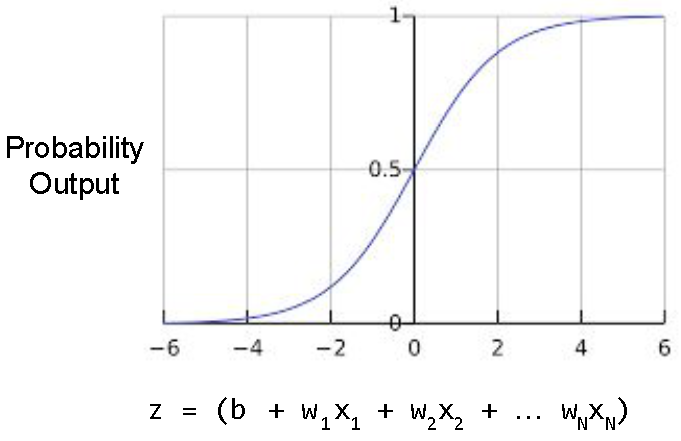
\includegraphics[width=0.5\textwidth]{fig/2-fundamentacao/aprendizado/probabilidade_output.png}
                \fonte{\cite{MachineL6:online}}
                \label{fig:probabilidade_output}
            \end{figure}